% DO NOT COMPILE THIS FILE DIRECTLY!
% This is included by the other .tex files.

\begin{frame}[t,plain]
\titlepage
\end{frame}

\begin{frame}
    \frametitle{Building blocks to support movies in MISP}
    MISP has no structures to express anything related to movie. 
    Let's fix that!
    \pause

    \vspace{1em}
    Tasks for this session:
    \begin{itemize}
        \item Movie genres (\texttt{Taxonomy})
        \item Movie sub-genres matrix (\texttt{Galaxy matrix})
        \item Movie and its details (\texttt{MISP Object})
        \item Get IMDB score when hovering (\texttt{hover-enrichment module})
        \item Get movie details from a title (\texttt{persistent-enrichment module})
    \end{itemize}
\end{frame}

\begin{frame}
    \frametitle{Movie genres - Taxonomy}
    \url{https://www.imdb.com/feature/genre/}
    \begin{center}
        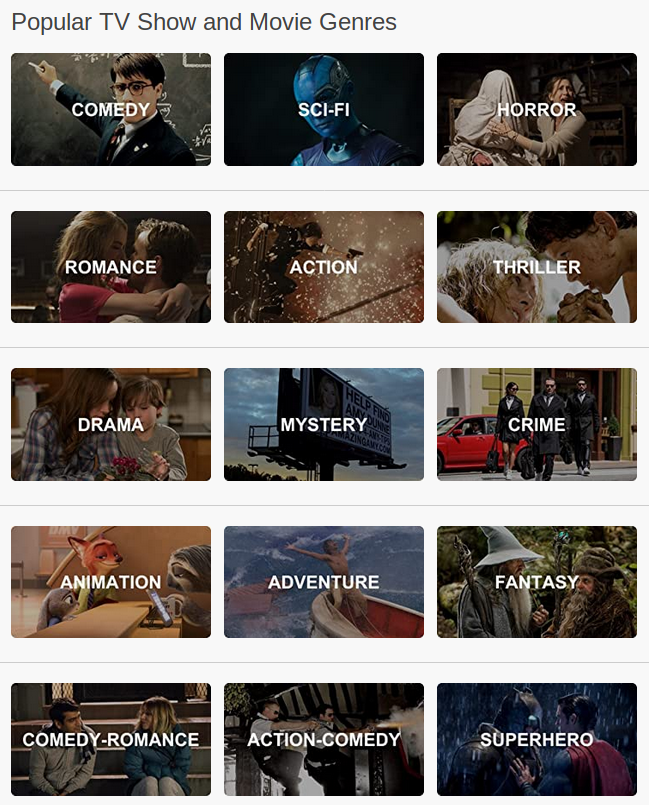
\includegraphics[scale=0.25]{pics/movie-genre}\\
    \end{center}
\end{frame}

\begin{frame}
    \frametitle{Movie subgenres - Galaxy matrix}
    \url{https://en.wikipedia.org/wiki/List_of_genres}
    \begin{center}
        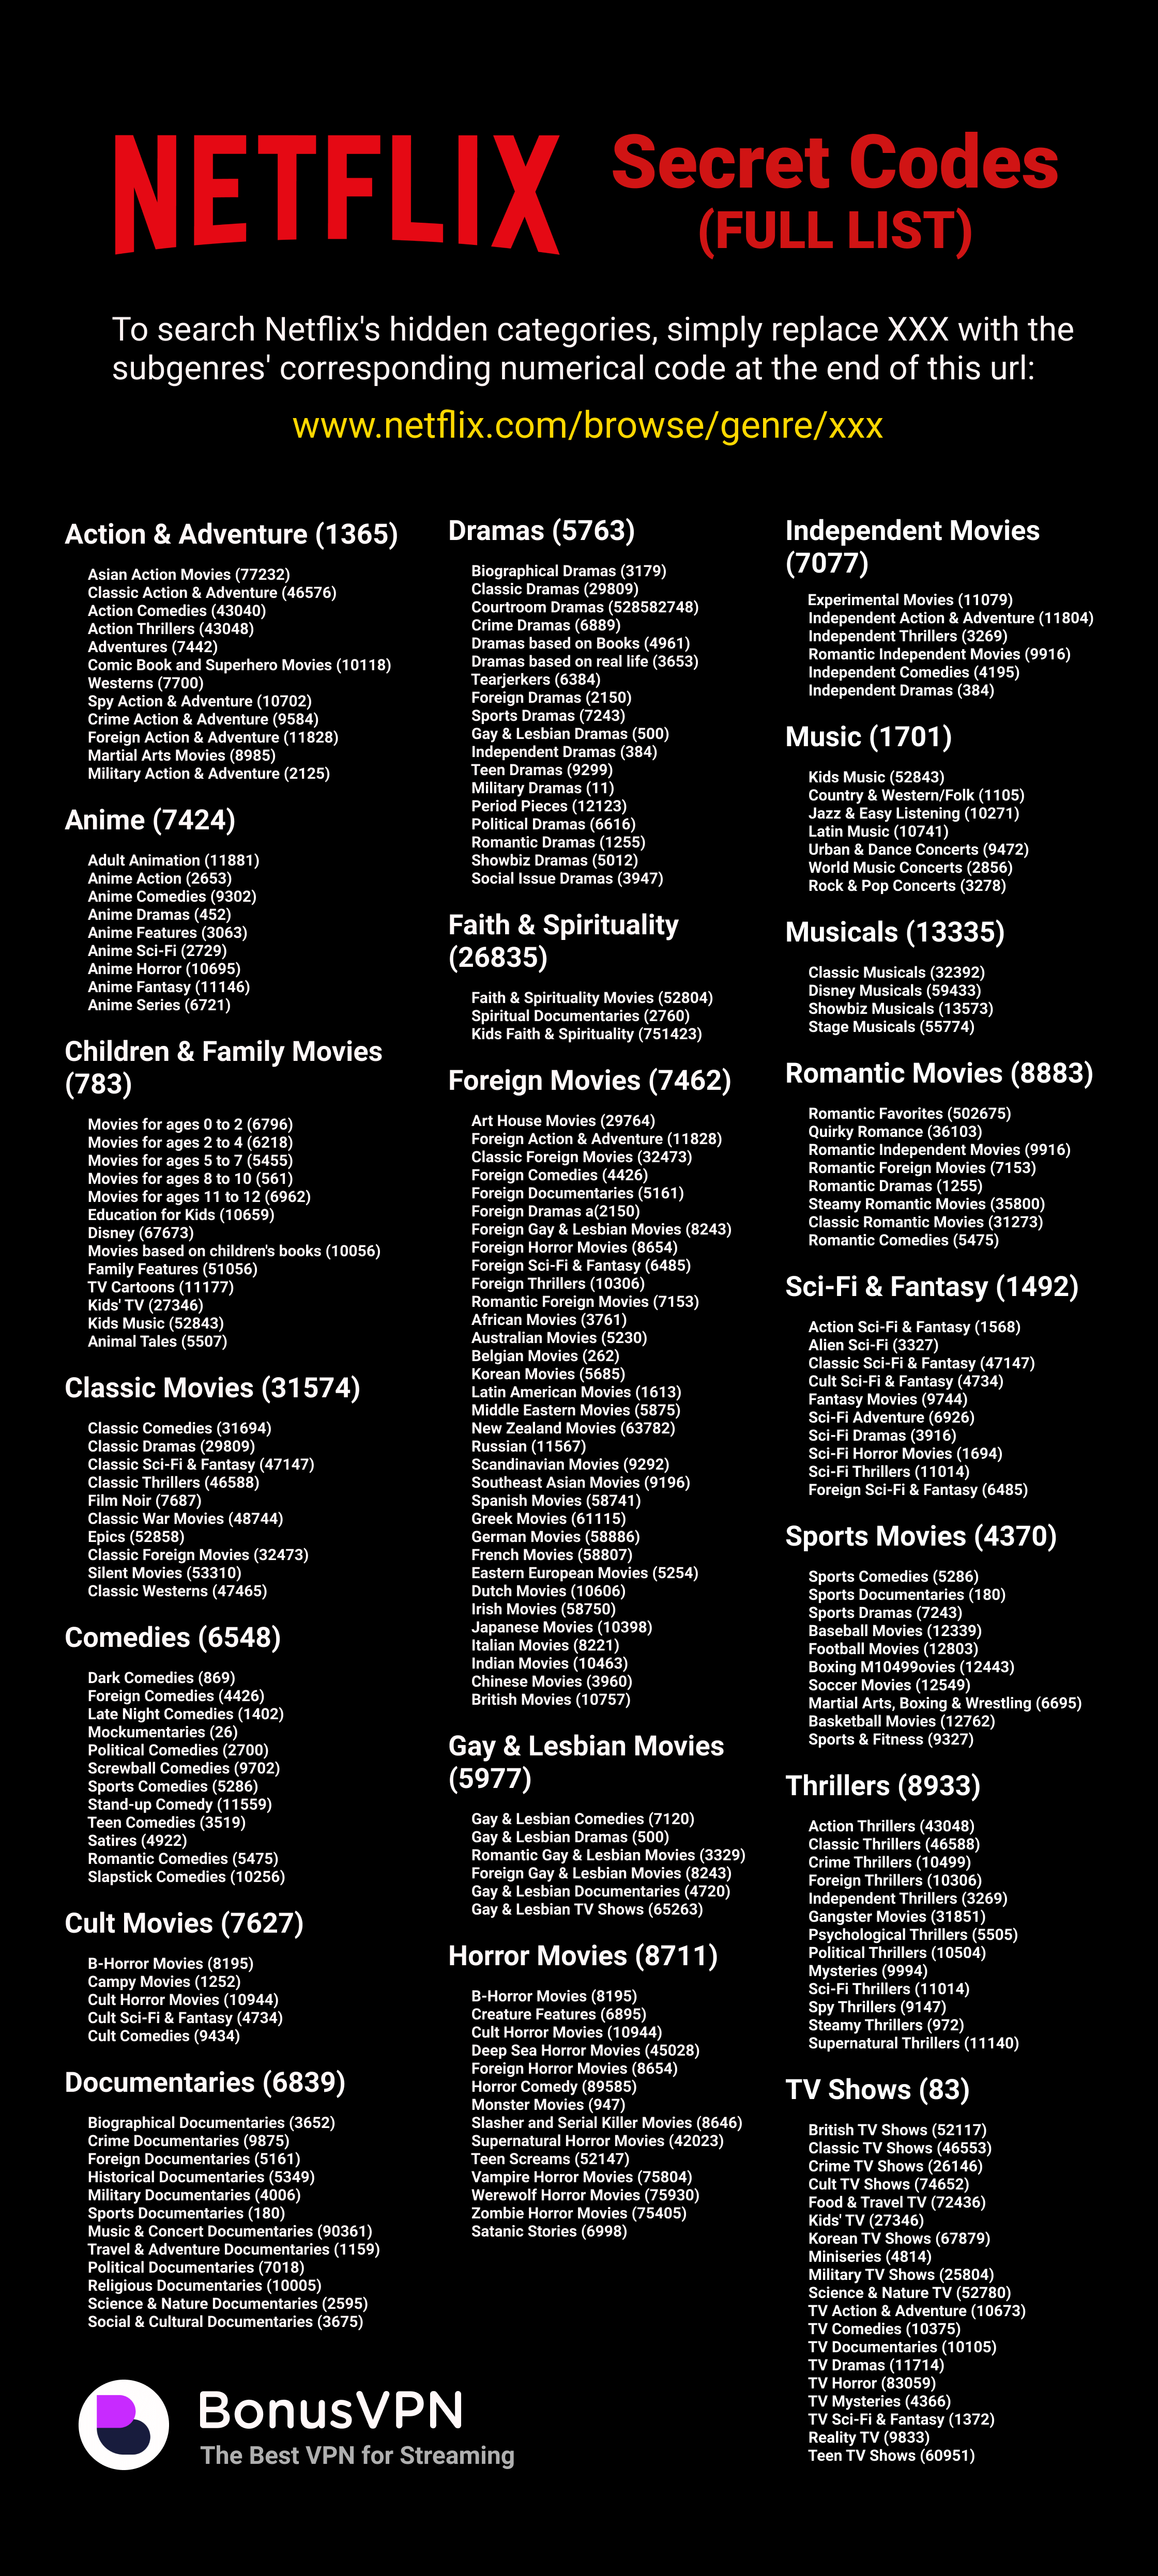
\includegraphics[scale=0.12]{pics/movie-subgenre}
    \end{center}
\end{frame}

\begin{frame}
    \frametitle{Movie \& details - MISP Object}
    \begin{center}
        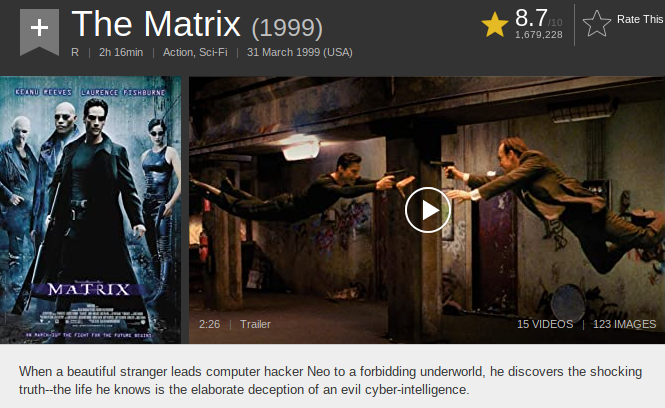
\includegraphics[width=0.70\linewidth]{pics/movie-details}
    \end{center}
    Movie fields:
    \begin{itemize}
        \item \texttt{title}
        \item \texttt{plot}
        \item \texttt{release-date}
        \item \texttt{duration}
    \end{itemize}
\end{frame}

\begin{frame}
    \frametitle{Movie IMDB score - Hover misp-module}
    \begin{center}
        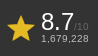
\includegraphics[width=0.3\linewidth]{pics/movie-score}
    \end{center}
    \begin{enumerate}
        \item From a movie title, fetch the associated score from IMDB
        \item Return the score as is
    \end{enumerate}
    \vspace{1em}
    Useful library: \url{https://imdbpy.github.io/}
\end{frame}

\begin{frame}
    \frametitle{Movie details from title - Persistent enrichment misp-module}
    \begin{center}
        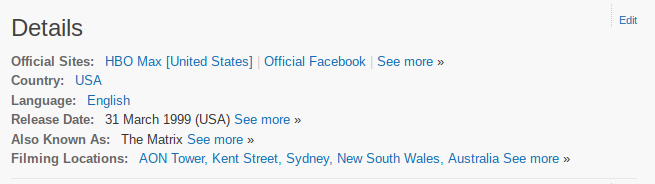
\includegraphics[width=0.85\linewidth]{pics/movie-details2}
    \end{center}
    \begin{enumerate}
        \item From a movie title, fetch additional information from IMDB
        \item Create a MISP Object with the details
        \item Include a reference from the create object to the enriched original attribute
    \end{enumerate}
    \vspace{1em}
    Useful library: \url{https://imdbpy.github.io/}
\end{frame}

\begin{frame}
    \frametitle{Example of solutions}
    \begin{itemize}
        \item \texttt{Taxonomy}: {\tiny \url{https://github.com/MISP/misp-taxonomies/tree/training-ex-movie}}
        \item \texttt{Galaxy matrix}: {\tiny \url{https://github.com/MISP/misp-galaxy/tree/training-ex-movie}}
        \item \texttt{MISP Object}: {\tiny \url{https://github.com/MISP/misp-objects/tree/training-ex-movie}}
        \item \texttt{Hover module}: {\tiny \url{https://github.com/MISP/misp-modules/tree/training-ex-movie}}
        \item \texttt{Persistent module}: {\tiny \url{https://github.com/MISP/misp-modules/tree/training-ex-movie}}
    \end{itemize}
\end{frame}
